\documentclass[11pt]{article}
\usepackage[margin=1in]{geometry}
\usepackage{amsmath,amssymb}
\usepackage{booktabs}
\usepackage{graphicx}
\usepackage{array}
\usepackage{longtable}
\usepackage{enumitem}
\usepackage{xr}
\usepackage[hidelinks]{hyperref}
\hypersetup{pdfauthor={Jiahao Wu; Amol Yerudkar; Carmen Del Vecchio},pdftitle={Computational Companion for Update-Rate-Constrained Semi-Markov Actor--Critic Learning for Probabilistic Boolean Control Networks},pdfsubject={Benchmark specifications, evaluation protocols and numerical evidence}}
\externaldocument{article_labels}

\newcommand{\E}{\mathbb{E}}
\newcommand{\Prob}{\mathbb{P}}
\newcommand{\R}{\mathbb{R}}
\newcommand{\N}{\mathbb{N}}
\newcommand{\1}{\mathbf{1}}
\newcommand{\Tbar}{\overline{T}}
\newcommand{\Gbar}{\overline{G}}
\newcommand{\Cbar}{\overline{C}}
\newcommand{\norm}[1]{\left\lVert #1 \right\rVert}
\newcommand{\abs}[1]{\left\lvert #1 \right\rvert}
\newcommand{\diag}{\mathop{\mathrm{diag}}}
\newcommand{\tr}{\mathop{\mathrm{tr}}}
\newcommand{\st}{\mathrm{s.t.}}
\newcommand{\proj}{\Pi}

\renewcommand{\thetable}{C\arabic{table}}
\renewcommand{\thefigure}{C\arabic{figure}}
\setlength{\emergencystretch}{3em}
\setlength{\tabcolsep}{4pt}
\renewcommand{\topfraction}{0.9}
\renewcommand{\bottomfraction}{0.8}
\renewcommand{\textfraction}{0.08}
\renewcommand{\floatpagefraction}{0.8}

\title{Computational Companion for\\[0.5ex]
\large Update-Rate-Constrained Semi-Markov Actor--Critic Learning for Probabilistic Boolean Control Networks}
\author{Jiahao Wu, Amol Yerudkar, and Carmen Del Vecchio}
\date{}

\begin{document}
\maketitle

\noindent
This guide specifies the computational models, evaluation conventions, numerical procedures and saved-output interpretation for the accompanying software. It contains implementation documentation and empirical records, not the article or its theoretical development. The command reference distinguishes saved-output export, numerical evaluation, training and certificate checking; access requirements and tested coverage are documented separately. PBCN denotes probabilistic Boolean control network, SMDP denotes semi-Markov decision process, PD-SMAC denotes primal-dual semi-Markov actor--critic, TT-AC denotes time-triggered actor--critic, DDQN+PER denotes double deep Q-network learning with prioritized experience replay, Macro-Q denotes macro-action Q-learning, and PD-SMAC-FA denotes the first-arrival primal-dual semi-Markov actor--critic adaptation. TD denotes temporal difference, ODE denotes ordinary differential equation, LP denotes linear program, and KKT denotes Karush--Kuhn--Tucker. The models and protocols are grouped by application, while the main text introduces the heterogeneous-dwell mechanism first. Section~C2.5 collects material provenance and reproduction qualifications.

\section*{C1. Notation and evaluation conventions}
\label{comp:sec:notation}

Table~\ref{comp:tab:notation_clocks} identifies the state, action, duration and metric quantities used by the numerical routines. Scores accumulate locally during a hold and return with its final state. Plant indices count physical transitions, decision indices count completed holds, episode indices count resets, and deterministic mean-field iterations count expected parameter updates.

\begin{table}[htbp]
\caption{Notation for interpreting the computational specifications and numerical records.}
\label{comp:tab:notation_clocks}
\centering
\begingroup
\small
\renewcommand{\arraystretch}{1.12}
\begin{tabular}{@{}p{0.27\linewidth}p{0.68\linewidth}@{}}
\toprule
Symbols & Meaning \\
\midrule
$t$, $k$, $t_k$ & Plant index, controller-decision index, and trigger instant. These differ from the fast critic and slow actor analysis clocks. \\
$X(t),U(t),X_k$ & Plant state, applied input, and trigger state $X(t_k)$. \\
$A_k=(u_k,\tau_k)$, $\tilde\tau_k$ & Selected macro-action and realized duration. Its components and $t_k$ are generally random. Complete holds have $\tilde\tau_k=\tau_k$ and $t_{k+1}=t_k+\tau_k$. \\
$P_u$, $\bar P^a$, $P_\theta$ & Plant-step, complete-hold, and fixed-policy trigger kernels. \\
$s$, $r_u=P_us_u$, $G$, $\widehat G_k$ & Post-transition score, its one-step expectation, complete-hold expected reward, and realized interval sum. \\
$d_\theta$, $\mu_\theta$ & Trigger-state and trigger state--action distributions, not plant-step occupation distributions. \\
$\Gbar$, $\Cbar$, $\Tbar$ & Reward, expenditure, and duration per trigger interval. Their ratios give plant-time rates $\eta$ and $\kappa$. \\
$c(a)$, $\nu$, $\widehat\nu_k$ & Per-decision update expenditure, excess numerator $\Cbar-\Gamma\Tbar$, and sample $c(A_k)-\Gamma\tilde\tau_k$. Input penalties in $s$ instead accrue per plant step. \\
$\theta$, $W$, $v$, $\vartheta_e$ & Actor coordinates, stored logit or actor-weight array, critic coordinates, and recorded softmax temperature. The numerical map from $W$ to the policy is stated in Section~C2.4. \\
$\pi_{\theta_{\rm out}}$, $\omega_{\theta_{\rm out}}$ & Saved stochastic policy and its separately evaluated greedy extraction. \\
$r=\kappa-\Gamma$, $R_{\rm pri}$ & Signed rate residual and nonnegative primal violation $\max\{0,r\}$, separate from the reward vectors $r_u$. \\
$T_{\rm cap}$, $K$, $A$, $F_H$ & Stopping time capped by the horizon, initiated holds, scalar input exposure, and failure indicator. The scalar $A$ is not $A_k$ or the advantage $A_{\theta,\lambda}$. \\
$h_{\theta,\lambda}$, $h^{\mathrm r}_{\theta,\lambda}$ & Stationary-mean and reference-state value normalizations. The state $i_0$ is fixed. The estimate $\hat\eta_k$ tracks $\eta_{\lambda_k}(\theta_k)$, not $\eta(\theta_k)$. \\
\bottomrule
\end{tabular}
\endgroup
\end{table}

\begingroup
\clubpenalty=10000
A fixed-horizon rollout evaluates post-transition states $X(1),\ldots,X(H)$. Hit probability records whether at least one evaluated state enters the target; first-target-arrival time is the first such index. The 28-node and 70-node evaluators use $H+1$ for failure, and their means include these codes. Writing $N_{\rm ev}$ for the number of evaluated paths, the restricted failure-coded mean is
\[
 \overline T_{\rm code}=N_{\rm ev}^{-1}\!\sum_{\ell:\,\mathrm{hit}}T_\ell+(H+1)(1-\widehat p_{\rm hit}).
\]
It is not uncensored mean hitting time. A successful-only mean is undefined if there are no hits. In the stopping experiment, $\overline T_{\rm code}=\overline T_{\rm cap}+1-\widehat p_{\rm hit}$, including initial targets at time zero. In the persistent experiments, first-visit coding does not change the executed horizon $H$. Target occupancy and task-reward rate are
\[
 \frac1H\sum_{t=1}^{H}\1_{\{X(t)\in\mathcal X_T\}},
 \qquad
 \frac1H\sum_{t=1}^{H}s(X(t),U(t-1)).
\]
For $K_H$ updates at executed-interval starts, including the initial update but excluding a new update at $H$, the rate is $K_H/H$ and its residual is $K_H/H-\Gamma$. The final hold has $\tilde\tau_k=\min\{\tau_k,H-t_k\}$. Scheduled and realized mean holds are $K_H^{-1}\sum_{k<K_H}\tau_k$ and $H/K_H$, respectively. A fixed hold gives $K_H=\lceil H/\tau\rceil$. Thus $H=28,\tau=5$ gives rate $6/28$, whereas $H=20,\tau=6$ gives rate $4/20$. All 28-node and 70-node rows report realized holds; periodic row names identify scheduled durations. Ratios do not commute with averaging. First-arrival means use recorded stopping totals and the stratified initial law described below.\par
\endgroup

Percentile intervals use 20,000 whole-unit resamples with linear quantile interpolation. Learned comparisons resample independent training-seed means, while fixed-policy comparisons resample rollouts. The 28-node continuation contrasts use paired whole-path indices. These pointwise, model/protocol-conditional intervals quantify sampling variation without multiplicity adjustment. Main Section~7.1 summarizes the uncertainty units. Learned sample deviations use four, five or ten training-seed means, with divisors three, four or nine; fixed melanoma population deviations use 480 or 1500 rollout values. Stored within-policy rollout standard errors are sample deviations divided by the square root of the rollout count. These units are not interchangeable. The rate residual in main Eq.~\textup{(\ref*{eq:finite_horizon_tradeoff_metrics})} differs from the interval numerator $\widehat\nu_k$, and feasibility of a mean does not establish individual seed or rollout feasibility.

\section*{C2. Benchmark models and essential protocols}
\label{comp:sec:benchmarks}

\subsection*{C2.1 Lactose first arrival and the separate mean-field diagnostic}
\label{comp:sec:lactose}
The nine-gene model has $2^9$ states, inputs $\mathcal U_{\mathrm{lac}}=\{0,1\}^2$, and complete holding times $\mathcal T_{\mathrm{lac}}=\{1,\ldots,5\}$. Table~\ref{comp:tab:lactose_update_rules} retains its update laws, with $X_i^+=X_i(t+1)$ and unshifted variables evaluated at $t$. The ON target is $\bar X_e=(1,1,1,1,1,1,0,1,1)$. Main Table~\ref*{tab:medium_results} compares first-arrival references, time-augmented Macro-Q and episodic PD-SMAC-FA. The interpretation concerns the current stopping protocol. Section~C2.5 distinguishes its records from unrecovered historical results.

\begin{table}[htbp]
\caption{Boolean update laws for the 9-gene lactose-operon PBCN benchmark.}
\label{comp:tab:lactose_update_rules}
\centering
\small
\setlength{\tabcolsep}{4pt}
\renewcommand{\arraystretch}{1.05}
\begin{tabular*}{0.96\textwidth}{@{\extracolsep{\fill}}c l c c l c@{}}
\toprule
Node & Update law & Prob. & Node & Update law & Prob. \\
\midrule
$X_1^+$ & $\neg X_7 \wedge X_3$ & $1$ & $X_6^+$ & $X_1$ & $1$ \\
$X_2^+$ & $X_1$ & $1$ & $X_7^+$ & $\neg X_4 \wedge \neg X_8$ & $1$ \\
$X_3^+$ & $\neg U_1$ & $1$ & $X_8^+$ & $X_4 \vee X_5 \vee X_9$ & $1$ \\
$X_4^+$ & $X_5 \wedge X_6$ & $1$ & $X_9^+$ & $\neg U_1 \wedge (X_5 \vee U_2)$ & $0.6$ \\
$X_5^+$ & $\neg U_1 \wedge X_2 \wedge U_2$ & $0.7$ & $X_9^+$ & $X_9$ & $0.4$ \\
$X_5^+$ & $X_5$ & $0.3$ &  &  &  \\
\bottomrule
\end{tabular*}
\end{table}


\paragraph{First-arrival protocol.}
States are binary-indexed with $X_1$ most significant, inputs are ordered $(0,0),(0,1),(1,0),(1,1)$, and durations increase within each input. Every coordinate updates synchronously; the choices at nodes 5 and 9 are independent at each plant step. The physical transition law is not made absorbing. Instead, target observation terminates the episode, including an observation inside a hold. Initial states are uniform on all 512 states. The target has initial mass $1/512$ and yields success with $T_{\rm cap}=K=A=0$. No decision or learning update is generated by that event.

The horizon is 100 plant steps. A hit on step 100 is success; otherwise failure incurs the terminal penalty 100. Each initiated hold incurs one controller update, even when cut short, but neither an unused remainder nor termination incurs an extra update. Only executed steps contribute to $A=\sum\|u\|_1$ and $T_{\rm cap}$. The objective is $J=\E[T_{\rm cap}+0.01A+100F_H]$, with numerator constraint $\E[K]-0.40\E[T_{\rm cap}]\leq0$ for constrained rows. The failure-inclusive coded time is $T_{\rm cap}+F_H$; it is not used in the objective's elapsed-time term or the rate denominator. Successful-only time conditions on $F_H=0$ and retains initially targeted states.

\paragraph{Model-based references.}
At a nonterminal pair $(x,r)$, where $r$ is remaining horizon, the killed one-step kernel $P_u^\circ$ deletes transitions into the target. Powers through $\min\{\tau,r\}$ describe survival, while first-hit probabilities determine the realized duration $\ell$. The immediate expected cost is $(1+0.01\|u\|_1)\E[\ell]+100\Pr(\text{horizon failure during this hold})$. Continuation occurs only after complete survival of a hold with positive remaining horizon. This construction accounts for interruption within a hold rather than using only its endpoint transition matrix.

Separate backward dynamic programs optimize the time-triggered and complete macro-action sets. Among actions within $10^{-10}$ of minimum cost, they minimize expected remaining updates, then use canonical action order. Independent initial-law evaluations agree within $10^{-8}$. The constrained reference uses nonnegative expected decision occupations on the time-augmented model, with killed-kernel flow and coefficients $1-0.40\E[\ell]$ for the budget. After minimizing $J$, a second program minimizes expected updates subject to cost at most $J^\star+10^{-10}$. All twenty actions remain available at each of the 17,044 structurally reachable pairs, producing 340,880 variables. Zero-occupation rows use the first canonical action.

Small occupation probabilities require numerical care. The solve uses $z=2^{20}y$ and re-evaluates the recovered policy. Independent forward propagation and Bellman dual potentials verify the flow, recovered moments and both optimization stages. The recovered-moment discrepancy is below $2\times10^{-13}$, and the independently reconstructed secondary dual gap is below $3\times10^{-12}$. Unscaled recovery and a raw secondary solver dual that failed their tolerances are excluded from active evidence. The primary budget multiplier is $0.005675779$ for $J+\lambda(\E[K]-0.40\E[T_{\rm cap}])$, not for a continuing rate constraint. Numerical reference certification does not identify this unrestricted class with the compact actor family.

\paragraph{Learned stopping policies.}
Macro-Q stores $Q(x,r,a)$, initially zero. Its target is $\ell+0.01\|u\|_1\ell+100F_{\rm terminal}+\min_{a'}Q(x',r-\ell,a')$, with zero bootstrap at termination and discount one. The learning rate at a pair-action's next visit is $0.5/(1+n)^{0.6}$, where $n$ is its prior visit count. At episode $e\in\{1,\ldots,5000\}$, exploration is $\max\{0.05,1-e/3500\}$, uniform over twenty actions; otherwise the lowest-index minimizing action is used. Its final table is evaluated greedily and has no update constraint.

PD-SMAC-FA uses temperature-one softmax rows $W(x,r,:)\in\mathcal C_{12}$, initialized at zero, a zero-initialized tabular critic $V$, and $\lambda_0=0.1$. With $d_e=(1+e/1000)^{-0.6}$, its actor, critic and dual gains are $0.02d_e$, $0.1d_e$ and $0.005d_e$. The actor and multiplier are frozen during an episode. The critic is updated online with
\[
 \delta=-\ell-0.01\|u\|_1\ell-100F_{\rm terminal}
 -\lambda(1-0.40\ell)+V(x',r-\ell)-V(x,r),
\]
where terminal bootstrap is zero. The actor accumulates the sum of TD-score contributions and applies one projected end-of-episode update, without dividing by $K$ or $T_{\rm cap}$. The multiplier becomes $\proj_{[0,50]}(\lambda+0.005d_e(K-0.40T_{\rm cap}))$. There is no continuing average-reward estimate in this adaptation. Initially targeted episodes advance the episode index without actor, critic or dual increments.

Each method uses ten training seeds and 5000 episodes per seed. Macro-Q executes 3,452,360 plant steps and PD-SMAC-FA 3,013,585, so equal episode budgets do not imply equal interaction budgets. Their actual plant and decision counts are recorded rather than equated to the horizon cap. Checkpoints at episodes 1000, 2000, 3000, 4000 and 5000 retain full parameters and critic or Q-table information. Each saved policy is evaluated with four independent trajectories from each state, giving 2048 equally weighted rollouts per seed. Plant tapes are paired across methods and policy modes, independently of training. The final checkpoint supplies the table endpoint; no earlier checkpoint is selected for better performance. The stochastic PD-SMAC-FA row is primary, and its greedy extraction is evaluated separately.

Within a seed, rate is $\sum K/\sum T_{\rm cap}$, scheduled mean hold is $\sum_k\tau_k/\sum K$, and realized mean hold is $\sum T_{\rm cap}/\sum K$. The initially targeted rollouts contribute zeros to totals; their individual ratios are undefined. Across seeds, arithmetic means and sample standard deviations are reported, with whole-seed percentile bootstrap intervals using 20,000 resamples. A mean of seedwise rates is not their pooled ratio, and the reciprocal of a mean rate is not a mean realized hold.

\begin{table}[tbp]
\centering\footnotesize
\textbf{Additional first-arrival metrics.}\\[3pt]
\setlength{\tabcolsep}{3pt}
\begin{tabular*}{\textwidth}{@{\extracolsep{\fill}}lrrrr@{}}
\toprule
Policy & \shortstack{Failure-coded\\time} & \shortstack{Successful-only\\time} & \shortstack{Scheduled\\hold} & \shortstack{Realized\\hold} \\
\midrule
\shortstack[l]{Time-triggered\\exact reference} & $5.688$ & $5.688$ & $1.000$ & $1.000$ \\[2pt]
\shortstack[l]{Macro-action\\exact reference} & $5.688$ & $5.688$ & $2.402$ & $1.899$ \\[2pt]
\shortstack[l]{Constrained macro\\exact reference} & $5.688$ & $5.688$ & $2.996$ & $2.500$ \\[2pt]
Macro-Q & $64.137 \pm 4.048$ & $32.037 \pm 4.610$ & $1.716 \pm 0.024$ & $1.681 \pm 0.024$ \\[2pt]
\shortstack[l]{PD-SMAC-FA\\stochastic} & $55.970 \pm 0.989$ & $40.349 \pm 0.955$ & $2.811 \pm 0.014$ & $2.753 \pm 0.014$ \\[2pt]
\shortstack[l]{PD-SMAC-FA\\greedy} & $54.462 \pm 6.394$ & $39.851 \pm 6.063$ & $1.413 \pm 0.030$ & $1.385 \pm 0.027$ \\[2pt]
\bottomrule
\end{tabular*}
\end{table}

All ten stochastic PD-SMAC-FA endpoints meet the empirical budget, whereas every greedy extraction and every Macro-Q endpoint exceeds it. The stochastic mean success probability is $0.742432$ and its mean cost is $82.020720$, well above the exact reference cost near $5.737437$. All final stochastic multipliers are zero. Supplemental exact evaluations of these same saved actors confirm negative expected budget numerators, but no actor-gradient estimate is supplied, so actor-stationarity entries remain undefined rather than zero. Neither inactive constraints nor zero complementarity establish a KKT point or a convergence guarantee. The 100,000 training episodes and 307,200 evaluation rollouts retain their different statistical roles.

\paragraph{Separate continuing diagnostic.}
The separate continuing mean-field diagnostic constructs 20 input--hold kernels on the 168-state closed one-step image, ordered by their binary state indices. Exhaustive transition checks recover this image from all 512 states. The common support graph of full-support actors is strongly connected and has self loops, so their trigger kernels are irreducible and aperiodic. The score is $s(x^+,u)=\1_{\{x^+=\bar X_e\}}-0.01\|u\|_1$, with one unit of update expenditure per hold and budget $\Gamma_{\rm lac}^{\rm conv}=0.25$. The actor has temperature one and every logit row belongs to $\mathcal C_{12}$ from \hyperref[comp:sec:actor_geometry]{Section~C2.4}.

Strict feasibility holds in this actual actor domain. At every state, assign logit $4$ to each of the four actions with duration $5$ and logit $-1$ to the remaining 16 actions. Each row sums to zero and lies strictly inside the box. Its state-independent duration law gives
\[
 \Tbar=\frac{5e^5+10}{e^5+4}>4,
 \qquad \kappa=\Tbar^{-1}\approx0.20265934<0.25.
\]
The invariant-law solve independently gives the same rate and a feasibility margin $0.04734066$. By contrast, the archived budget-$0.20$ illustration has an empty feasible full-support actor class because $\Tbar<5$ and $\kappa>0.20$. Its trace and former proxy are retained as historical records, not used in the revised diagnostic.

The calculation makes 620 simultaneous actor/dual updates using the current pair in both increments,
\[
 \theta^+=\proj_\Theta(\theta+10g),\qquad
 \lambda^+=\proj_{[0,20]}\bigl(\lambda+0.50(\kappa-0.25)\bigr),
 \qquad g=\nabla_\theta\eta_\lambda(\theta).
\]
The projection is the Euclidean zero-sum-box projection, not centering followed by clipping. Initial logits are independent normal draws with standard deviation $0.001$, followed by this projection, and $\lambda_0=0.1$. NumPy PCG64 uses the SeedSequence key $(20260917,11,20,3,0,250,0,0,0)$. No tuning or residual-based endpoint selection is used. Every iterate from 0 through 620 is saved; Figure~\ref{comp:fig:lactose_convergence} displays every fifth iterate.

Each iterate uses its stochastic-policy invariant law and a differential-value solve normalized at the first state of the ordered closed image, whose local code index is 0. This is the reference state $i_0$ of the main text and gives 167 reduced indicator coordinates. The stored image identifies it with the all-zero Boolean state. The value equation uses $\eta_\lambda=\eta-\lambda\kappa$; the task-reward rate $\eta$ and Lagrangian $\eta-\lambda(\kappa-0.25)$ are recorded separately. The rate Lagrangian differs from $\eta_\lambda$ only by the constant $\lambda\Gamma_{\rm lac}^{\rm conv}$, so these two penalized objectives have the same actor gradient. The largest invariant-law and Poisson-equation residuals over the saved trace are $1.7\times10^{-15}$ and $6.2\times10^{-10}$, below the prescribed tolerances $10^{-10}$ and $10^{-9}$. Independent invariant-law and augmented Poisson solves check all 621 saved pairs, and a separate execution reproduces the complete numerical trace.

The endpoint task-reward rate is $0.98984705$, target occupancy is $0.99984705$, and update rate is $0.20001946$. The signed rate residual is $-0.04998054$, with multiplier zero. The rate first falls below the budget at iteration 24, and the multiplier reaches zero at iteration 63. Its maximum is $0.912681$, so the artificial upper bound is never active. The separate residuals defined in main Section~\ref*{sec:convergence} satisfy
\[
 R_{\rm act}=1.59425\times10^{-4},\qquad
 R_{\rm pri}=0,\qquad R_{\rm comp}=0.
\]
The projected actor residual exceeds the declared $10^{-5}$ threshold, so the endpoint is not classified as near-stationary. The inactive constraint and zero complementarity do not establish a KKT point. The complementary advantage calculation in Section~C2.4 gives $R_{\rm adv}=0.001947516672$ at this same endpoint and multiplier. It is evaluated from the lactose model and is not a cross-model performance score. Exact-model constant-gain integration does not verify sampled critic tracking, stochastic convergence, isolated equilibria, or global optimality.

\subsection*{C2.2 Melanoma models, features, and provenance}
\label{comp:sec:melanoma}
Both models regulate WNT5A-OFF through pirin-directed intervention, with binary input and score $s(x^+,u)=\1_{\{x^+_{i_w}=0\}}-0.06u$. All gene-coordinate indices in this subsection use the zero-based code convention, with pirin $i_p=0$ and WNT5A $i_w=1$. The 28-node model uses the transient exclusive-or (XOR) intervention
\[
 X_{i_p}(t+1)=\tilde f_{i_p}^{\sigma(t)}(X(t))\oplus U_p(t),
\]
while other coordinates follow the fitted stochastic predictor bank. The 70-node input $u=1$ instead forces pirin ON at the next step and evaluates downstream pirin-responsive rules with pirin ON; $u=0$ selects the baseline banks. These are different controlled transitions, not a matched network-size experiment.

The banks are fitted from frozen binary views of 31 Bittner samples. Row-wise two-means clustering is the documented workbook-reconstruction procedure; the independent 70-node primary-view derivation limitation is specified below. Weighted-gene ordering pads the seven-gene seed set. For each target, the six highest mutual-information predictors generate one-, two-, and three-predictor Boolean lookup rules. The two most accurate rules are retained, preferring shorter predictor sets in ties. The controlled bank adds pirin and retains pirin-containing rules; WNT5A uses the pirin-only rule and the next distinct such rule. Sampling weights are proportional to $\max\{10^{-3},\text{training accuracy}\}$. The reset pool contains five observed WNT5A-ON states and enforces $x_{i_w}=1$.

The compact feature is
\[
\chi_n(x)=\bigl[1,\;x_{i_w},\;x_{i_p},\;\{x_j:j\in J_w\},\;
\bar x,\;\bar x_{\mathcal R_p},\;s_{\mathcal R_p}(x)\bigr]^\top.
\]
The predictor coordinates $J_w$ enter $\chi_n$ in their stored order, with at most three entries. In the retained numerical records, $J_w=\{7\}$ contains only the coordinate for gene ID 357278. The set $\mathcal R_p=\{1,\ldots,n-1\}$ contains pirin-responsive coordinates. The symbols $\bar x$, $\bar x_{\mathcal R_p}$, and $s_{\mathcal R_p}(x)$ denote network mean activity, set mean activity, and its population-divisor standard deviation. TT-AC uses a logistic input actor with $\tau=1$; PD-SMAC uses action-specific linear softmax logits. Both use $\xi(x)=\chi_n(x)$, constant numerical gains, and greedy endpoint extraction. These are numerical feature approximations, distinct from the exact-realizability setting of the analysis. DDQN+PER is the time-triggered deep reference. Fixed-hold comparisons use $u\equiv1$ and every duration listed in Table~\ref{comp:tab:melanoma_protocol}. The gains, replay rules and evaluation streams for both models are specified below and in their separate configuration records.

The 28-node workflow uses the hash-verified 31-by-28 binary view and the baseline banks reconstructed from that view. The zero-based reset-row indices are $2,4,5,8,11$, sampled uniformly with their recorded multiplicities. The feature order is $[1,x_1,x_0,x_7,\bar x,\bar x_{\mathcal R_p},s_{\mathcal R_p}(x)]^\top$, so its dimension is seven. Each of the 20 runs executes 240 episodes and 6720 plant steps, with truncation of the final hold at step 28. Target visits do not terminate an episode. Parameters persist across resets, and actor--critic TD targets bootstrap from the physical state at the horizon, whereas the DDQN target has no terminal bootstrap.

The TT-AC actor, critic and average-reward gains are $0.01$, $0.04$ and $0.012$. The corresponding PD-SMAC gains are $0.004$, $0.02$ and $0.008$, with dual gain $0.008$, initial multiplier $0.1$ and no upper cap. The dual increment uses $1-\Gamma\tilde\tau_k$; actor weights are not projected. DDQN+PER has two 64-unit rectified-linear hidden layers, Adam step size $10^{-3}$, discount $0.98$, batch size 32 and replay capacity 5000. Priorities use exponent $0.6$ and offset $10^{-3}$; the importance exponent increases from $0.4$ to $1$. Replay draws are with replacement, with the maximum absolute pre-update TD error used for duplicate priority writes. Double-Q targets use online action selection and target-network evaluation; the target is synchronized every 100 plant steps. 

Training initialization, actions, plant draws, resets, replay and exploration use separate recorded random streams. Every 40 episodes, each saved actor is evaluated greedily and stochastically on 120 rollouts per training seed, with separate actor randomness and shared plant/reset tapes across methods and budgets. DDQN evaluation is greedy. The fixed references use the same four terminal tape blocks, giving 480 rollouts each. All terminal table entries and checkpoint-240 points share evaluation identifiers and raw outcomes. The endpoint files retain scheduled and executed holds, input exposure, task reward and controller-update counts. Reported learned means average the four seedwise estimates. Intervals use 20,000 paired whole-seed bootstrap samples; fixed-policy intervals instead resample rollouts. These uncertainty units are not interchangeable.

For stochastic PD-SMAC at budgets $0.25$, $0.40$ and $0.55$, the mean update rates are $0.245238$, $0.322024$ and $0.340253$, respectively; their mean occupancies are $0.640848$, $0.590476$ and $0.586756$. Seed 2 at budget $0.25$ has rate $0.254167$, exceeding its empirical limit; the other eleven stochastic budget--seed endpoints are feasible. The corresponding greedy endpoints are all feasible but are different policies. TT-AC's evaluated greedy paths all use $u=0$, whereas its stochastic mean occupancy is $0.416518$. The largest absolute pre-clipping TT-AC logit in training is $3.756128$, well inside the clipping threshold 30. No claim about exact stationary gradients, feature-actor isolation or stochastic convergence follows from these finite records.

All twelve greedy PD-SMAC endpoints have exactly the same WNT5A paths as the paired $u\equiv1$ reference on the observed terminal tapes. Five use both inputs, and all their zero-input steps occur after a first target visit. Full-state equality is not asserted. The fitted WNT5A rules depend on coordinate 7, not directly on pirin; timing and input changes can therefore leave the observed target trajectory unchanged without producing identical controllers. 

\paragraph{Paired training-budget control.}
At $\Gamma=0.40$, four paired paths for each of DDQN+PER, TT-AC and PD-SMAC continue to 1200 total episodes. Complete episode-240 states preserve actor/critic arrays and scalar types, Adam moments, target weights, replay priorities and ring positions, counters and random-stream offsets. Exact prefix and split-continuation checks establish pairing on the tested environment; Section~C2.5 records the hardware scope.

The DDQN schedules are $\epsilon(e)=\max\{0.05,1-e/(0.7\cdot240)\}$ and $\beta_{\rm PER}(e)=\min\{1,0.4+0.6e/240\}$. Their tails remain $0.05$ and 1; no schedule or counter restarts at episode 241. Other gains and the XOR model remain unchanged. The control adds 322,560 plant steps to the 80,640-step cohort prefix. Checkpoints at episodes 240, 480, 720, 960 and 1200 use 120 rollouts per seed and the same terminal evaluation tapes. Four paired path differences, not independent short/long samples, define each contrast. The 20,000-resample intervals use whole-path indices and linear quantiles. Fixed-reference blocks are reused without a new bootstrap. Additional validation replays are not statistical seeds.

Table~\ref{comp:tab:training_budget_sensitivity} gives both policy modes and paired changes. All forty PD-SMAC evaluations are empirically feasible, but the final stochastic seed-3 multiplier $0.0048$ has complementarity product $0.0006614286$. Stochastic TT-AC seed 2 loses $0.134524$ in occupancy. The preserved greedy mean ordering does not eliminate training-budget sensitivity or establish an optimized-method ranking.

The 70-node workflow uses the frozen gene-by-sample view in its manifest order, transposed to 31-by-70 for fitting. The reset-row indices are again $2,4,5,8,11$, retaining multiplicities. Both fitted rule banks, every local Boolean lookup row and the seven-feature ordering were checked against the specified model constructor. The baseline and controlled transitions reserve one independent plant draw per coordinate and physical step, including the bypassed forced-pirin coordinate. 

The 15 learned runs comprise five DDQN+PER, five TT-AC and five PD-SMAC runs at budget $0.40$. Each executes 300 episodes of 20 plant steps, without target termination, giving 6000 training interactions. Gains, average-reward updates and actor domains are those specified above for the biological implementations. The PD-SMAC action order is $(0,1),(0,2),(0,4),(0,6),(1,1),(1,2),(1,4),(1,6)$. The DDQN input is the full 70-bit state, with two 64-unit rectified-linear-unit (ReLU) hidden layers and two outputs. Online argmax selects the bootstrap action, the target network evaluates it, and horizon-terminal transitions have no bootstrap. Initial target weights equal the online weights, with copies every 100 plant steps. Adam uses step size $10^{-3}$ and its default moment and numerical constants.

Replay draws 32 samples with replacement from capacity 5000 after the buffer first reaches 32 entries. Sampling uses $p_i\propto q_i^{0.6}$ for positive stored priorities $q_i$, and normalized batch weights $(N_{\rm buf}p_i)^{-\beta}$, where $N_{\rm buf}$ is the current replay-buffer size and $\beta=\min\{1,0.4+0.6e/300\}$ in episode $e$. This $\beta$ is a replay importance exponent, not the critic gain $\beta_k$. Duplicate indices receive the largest absolute pre-update TD error plus $10^{-3}$, and new entries receive the current maximum priority. Exploration is $\epsilon_e=\max\{0.05,1-e/(0.7\cdot300)\}$; evaluation sets it to zero. Ties use the first canonical Q or softmax action, whereas TT-AC chooses $u=1$ at probability $1/2$. All five DDQN runs complete 5969 optimizer updates. 

Five training labels $0,\ldots,4$ use independent initialization, action, plant, reset, replay and exploration streams. Each stream is derived by SeedSequence and PCG64 from $(20260917,15,p,m,s,g,e,r,c)$, where the recorded purpose, method, seed, budget, checkpoint, rollout and component coordinates distinguish its use. Paired evaluation plant and reset streams set method and budget coordinates to zero. Evaluations every 50 episodes save both actor modes, except that DDQN is evaluated greedily. Each uses 300 rollouts, and fixed policies use all five terminal blocks. There are 90 saved checkpoints and 190 evaluation records covering 57,000 rollouts. Learned uncertainty uses five independent training-seed means with sample divisor four; fixed-policy uncertainty uses 1500 rollout outcomes with population divisor. Percentile intervals use 20,000 paired whole-seed bootstrap resamples for learned rows and a separate pooled-rollout bootstrap for fixed rows.

At the final checkpoint, every greedy TT-AC path uses $(1,1)$ and every greedy PD-SMAC path uses $(1,6)$. Both match the paired constant-input full-state trajectories. Their task-reward means equal $0.823767$, but their rates are 1 and $0.20$, respectively. The nominal-6 reference executes a final length-2 hold, so its realized mean hold is 5. These observations establish neither equality on unvisited states nor a timing-based regulation advantage. Stochastic TT-AC has mean occupancy $0.879833$, reward $0.824801$ and rate 1. Stochastic PD-SMAC has mean occupancy $0.865367$, reward $0.815323$ and rate $0.281167$; all five corresponding empirical rates satisfy the budget. Its endpoint multipliers are $0.0048,0.0016,0.0016,0,0$. The three positive-multiplier endpoints have nonzero empirical complementarity products; these finite-rollout quantities are not stationary certificates. Actor stationarity is uncomputed, not zero. The continuing tabular convergence results do not certify these reset feature implementations.



\subsection*{C2.3 Heterogeneous-dwell model and evaluation}
\label{comp:sec:heterogeneous}
The four encoded Boolean states are $S=(1,0)$, $B=(1,1)$, $O=(0,1)$, and $L=(0,0)$ in local coordinates $(Y,R)$, with target $\mathcal X_T^{\rm het}=\{S,B\}$. Both $Y$ and $R$ are Boolean coordinates in this encoding; the local $R$ is separate from the main paper's input-alphabet cardinality. In that state order the controlled kernels are
\[
P_0=\begin{bmatrix}
0.98&0.02&0&0\\
0.02&0.03&0.95&0\\
0&0.03&0.87&0.10\\
0&0&0.10&0.90
\end{bmatrix},\qquad
P_1=\begin{bmatrix}
0.15&0.10&0.75&0\\
0.95&0.05&0&0\\
0.02&0.78&0.20&0\\
0&0.20&0.70&0.10
\end{bmatrix}.
\]
A short repair input $u=1$ benefits boundary state $B$ but is harmful when retained at safe state $S$. The score is $s(x^+,u)=\1_{\{x^+\in\mathcal X_T^{\rm het}\}}-0.02u$, with holds $\{1,\ldots,5\}$, $c(a)=1$ and budget $0.30$. For $a=(u,\tau)$, write
\[
 Q_{ij}(a)=\bar P^a_{ij}=[P_u^\tau]_{ij},\qquad
 G_T(i,a)=\sum_{\ell=1}^{\tau}[P_u^\ell\1_{\mathcal X_T^{\rm het}}]_i,
 \qquad G(i,a)=G_T(i,a)-0.02u\tau.
\]
Each fixed duration enumerates all 16 state-dependent input maps. All 10,000 deterministic macro-policies are enumerated, with 3307 feasible policies, 2150 reducible policies and no multichain policy. The fixed one-step selector using $u=0$ at $S$ and $u=1$ elsewhere has recurrent class $\{S,B\}$ and transient states $O,L$. The numerical reference rates are obtained from their unique invariant laws and direct enumeration, separately from Bellman-solution existence arguments. For each objective, policies within $10^{-10}$ of its maximum are tied, then minimized in rate within $10^{-10}$ and ordered lexicographically in the canonical action indices. Both deterministic objectives select $S:(0,4)$, $B,O:(1,1)$ and $L:(1,2)$.

For either $g=G_T$ or $g=G$, the unrestricted stationary randomized benchmark solves
\[
 \begin{aligned}
 \max_{y\ge0}\quad &\sum_{i,a}y_{ia}g(i,a),\\
 \text{subject to}\quad
 &\sum_a y_{ja}-\sum_{i,a}y_{ia}Q_{ij}(a)=0\quad(j\in\{S,B,O,L\}),\\
 &\sum_{i,a}\tau(a)y_{ia}=1,\qquad \sum_{i,a}y_{ia}\le0.30.
 \end{aligned}
\]
Here $y_{ia}$ is decision occupancy per plant step, not a distribution summing to one. For a stationary policy it equals $\mu_\pi(i,a)/\Tbar(\pi)$, where $\mu_\pi$ and $\Tbar(\pi)$ are its trigger-level state--action distribution and mean duration. The local LP objective $g$ is a scalar macro-reward, whereas the diagnostic $g=\nabla_\theta L$ is an actor gradient. For positive state mass, recover $\pi(a\mid i)=y_{ia}/\sum_b y_{ib}$. All state masses are positive in both computed solutions. Independent invariant systems recover their objective and update rate. Validation checks all flow equations, duration normalization, nonnegativity, budget slack, dual feasibility and complementarity, and the primal--dual gap. A second LP algorithm and the independent selector dual
\[
 \min_{\rho\in\mathbb R,\,\lambda\ge0}\rho+0.30\lambda,
 \qquad \rho+\lambda\kappa_d\ge\eta_{g,d}\quad\text{for all 10,000 selectors }d
\]
also agree. The tolerances are $10^{-9}$ for flow and duration normalization, $10^{-10}$ for the budget, and $10^{-8}$ for objective agreement and primal--dual residuals. They are numerical checks, not formal exact-arithmetic certificates.

The occupancy LP gives $0.972661989233825$ with multiplier $0.121641615667607$. The penalized LP gives $0.971927385746528$ with multiplier $0.122138824356443$. They select the same policy in this model, randomizing between $(0,3)$ and $(0,4)$ at $S$ with probabilities $0.522864697003933$ and $0.477135302996067$. States $B,O,L$ use $(1,1),(1,2),(1,2)$, respectively. Both rates equal $0.30$ to numerical precision. These zero-containing distributions are unrestricted references, not optima over the compact full-support actor domain. Conditional safe-state randomization adjusts mean dwell while retaining short repair actions elsewhere.

The reset/annealed four-state training protocol uses ten independent seed labels $0,\ldots,9$, master entropy 20260917 and separate action, plant and reset streams. Each of 1200 episodes resets uniformly, then executes complete holds while elapsed plant time is below 295. Consequently an episode lasts 295--299 steps. The ten primary runs contain 3,559,683 plant steps and 881,857 decision updates. Initially $W=0$, the represented value is zero, $\hat\eta_0=0$ and $\lambda_0=0.1$. The implementation variable \texttt{eta}, saved as \texttt{critic\_eta}, estimates the penalized rate $\hat\eta$, not the evaluated task-reward rate $\eta$. At episode $e\in\{1,\ldots,1200\}$, the actor, critic, rate and dual gains are $(0.12,0.16,0.05,0.08)/(1+e/1000)^{0.6}$. Sampling uses $\operatorname{softmax}(W_i/\vartheta_e)$ and score $(e_a-\pi_i)/\vartheta_e$, with the temperature in Section~C2.4. The actor uses the true $B=12$ zero-sum-box projection. After the TD update, the critic is normalized by subtracting its value at $S$, and the multiplier uses $1-0.30\tau$ with cap 50. All plant transitions within a hold are retained. This finite reset-training profile is not asserted to satisfy the asymptotic multi-timescale hypotheses of the convergence results.

At episodes 300, 600, 900 and 1200, exact stationary systems evaluate the saved stochastic actor and its separate canonical greedy extraction, using no rollout noise. Complete-hold means are trigger-state weighted. Each policy satisfies $\kappa=1/\Tbar$, but the reciprocal of the across-policy mean hold is not the mean update rate. Figure~\ref*{fig:heterogeneous_dwell_tradeoff} and all gaps derive from unrounded saved outputs.

Only the penalized LP multiplier is objective-matched to the learner. Each stochastic policy is evaluated with its own saved multiplier and exact penalized differential value. All ten endpoints are feasible, and the largest unit-step projected rate-gradient residual is $1.106743\times10^{-7}$, below the declared $10^{-5}$ diagnostic threshold. Seed labels 1, 4 and 5 retain multipliers $0.004985$, $0.029908$ and $0.034893$ despite slack rates, with complementarity residuals $1.806344\times10^{-4}$, $2.520881\times10^{-3}$ and $1.245095\times10^{-3}$. The other seven multipliers are zero. No upper-cap update occurs. Low-temperature action concentration, not an active logit-box bound, accompanies these small actor residuals. Separate duration-scaled mappings are saved rather than inferred by linear rescaling. No multiplier or stationarity certificate is attached to a greedy extraction, and the finite diagnostics do not establish KKT convergence or global optimality.

\paragraph{Representation loss and exact ties.}
Separate exact rational primal--dual checks of the stored LP supports verify both unrestricted objectives without another optimization. For the witness, fix $p=0.5228627141649896$ as a terminating decimal and put $q=(1-p)/p$. At $S$, set
\[
 W_{(0,3)}=12,\quad W_{(0,4)}=12+\log q,\quad
 W_a=-\frac{24+\log q}{8}\quad(a\ne(0,3),(0,4)).
\]
At $B,O,L$, give actions $(1,1),(1,2),(1,2)$ logit 12 and the other nine entries $-4/3$. All rows sum to zero and lie in $\mathcal C_{12}$. The temperature-one softmax has full support; the actor is on a box face, not in its interior. Directed 384-bit dyadic arithmetic, stationary cofactors and independent high-precision solves enclose occupancy $0.972660987446361568$, reward $0.971926355944844560$ and rate $0.299999989999999907$. The entire rate enclosure is below $0.30$. These are mathematical-model numerical certificates, not learned outcomes.

For fixed temperature $\vartheta$, $W_{\vartheta}=\vartheta W$ represents the same witness. Both nominal $0.15$ and the stored binary64 temperature $1351079888211149/9007199254740992$ are checked. The original saved policies have feasible zero-sum representatives in this endpoint-temperature box. None represents the same policy inside the temperature-one box; their centered temperature-one magnitudes would reach approximately $45.55$--$55.95$.

For objective $J$, let $J_U$ be the unrestricted optimum, $J_\Theta$ the feasible optimum in the named actor family, $J_w$ the witness value and $\overline J$ the original cohort mean. Since $J_w\le J_\Theta\le J_U$, the endpoint-temperature family satisfies
\[
 0\le J_U-J_\Theta\le J_U-J_w,\qquad
 J_w-\overline J\le J_\Theta-\overline J\le J_U-\overline J.
\]
Outward bounds on representation loss are $1.001788\times10^{-6}$ for occupancy and $1.029802\times10^{-6}$ for reward. The corresponding finite-training shortfall brackets are
\[
 \begin{aligned}
 \text{Occupancy:}&\quad [0.011569274904816,0.011570276692281],\\
 \text{Reward:}&\quad [0.011876450252729,0.011877480054414].
 \end{aligned}
\] These deterministic bounds do not quantify population training uncertainty or identify a unique optimization cause. They are not assigned to the temperature-one family for the cold policies or to infeasible new endpoints.

The fixed-duration occupancy/reward pairs are $(0.926421867,0.922512036)$ at duration 3 and $(0.926281541,0.922850230)$ at duration 4. The former rate $1/3$ is infeasible. The two optimal deterministic ties have exactly shared occupancy $171957881/177554825$ and reward $1583657/1636450$; using hold 2 instead of 1 at $L$ reduces the rate by $100358/78124123$. The condition $P_1(L,S)=0$ makes the skipped decision redundant because the possible intermediate states keep input 1.

At three and six decimal places the original stochastic and greedy summaries coincide, but their means differ by approximately $(1.1194,1.1930,3.9224)\times10^{-9}$ in occupancy, reward and rate, and $8.9710\times10^{-8}$ in hold duration. Their sample-deviation differences are approximately $(2.0958,2.2342,6.5924)\times10^{-9}$ and $1.5251\times10^{-7}$, respectively. Mean hold separates at seven decimals as $4.0879243$ and $4.0879242$. Equality after rounding is not equality of policies.

\paragraph{Continuing sampled experiment.}
The additional study uses $\xi(S)=0$, $\xi(B)=e_1$, $\xi(O)=e_2$, $\xi(L)=e_3$ and exactly three critic coordinates. The update at $S$ is therefore zero in critic coordinates; updating four values and renormalizing is not substituted for this recursion. With global decision index $k$ starting at zero,
\[
 \begin{aligned}
 \beta_k&=0.16(1+k)^{-0.6},&\quad \beta_k^{(\eta)}&=0.05(1+k)^{-0.6},\\
 \alpha_k&=0.12(1+k)^{-0.9},& \zeta_k&=0.08(1+k)^{-0.9}.
 \end{aligned}
\]
Their required sums and square sums, constant rate/critic and dual/actor ratios, and vanishing slow/fast ratios hold. All right-hand sides use the same old iterate and the sampled complete-hold TD error. There is no critic projection, terminal mask, entropy term or exact-value feedback. The actor has fixed temperature one and the same $\mathcal C_{12}$ domain; $W_0=v_0=\hat\eta_0=0$, $\lambda_0=0.1$ and $\lambda\in[0,50]$. A single uniformly sampled initial state is followed by continuing holds without resets. The ten independent new stream labels $0,\ldots,9$ use master seed 20260919 and study coordinate 212.

Each path completes $10^6$ decisions. The cohort contains 30,466,939 plant steps and retains checkpoints $k=0,100,1000,5000,10000,25000,50000,100000,200000,400000,600000,800000,10^6$. Checkpoint evaluations do not consume training randomness. Independent reconstruction checks every sampled update; a preselected complete replay is validation, not an eleventh statistical seed. Tables~\ref{comp:tab:continuing_endpoints} and \ref{comp:tab:saved_policy_diagnostics} retain the distinct continuing and original protocols.

All final continuing stochastic policies are infeasible and fail the actor, primal and complementarity thresholds. Their mean rate-estimate absolute error is $0.001705$ and mean reference-value error is $0.243309$; no multiplier reaches the cap. Greedy extractions are feasible but do not certify the stochastic recursion. The scope in main Section~6.4 retains Assumption~\ref*{ass:critic_bounded} and the isolation requirement.

\begin{table}[htbp]
\caption{Essential evaluation profiles. The 28-node row describes the saved-policy experiment; its fixed holds use four paired terminal blocks totaling 480 rollouts. The 70-node fixed policies use five paired terminal blocks totaling 1500 rollouts. Fixed holds require no training. The lactose mean-field protocol is specified separately in \hyperref[comp:sec:lactose]{Section~C2.1}.}
\label{comp:tab:melanoma_protocol}
\centering
\begingroup
\small
\renewcommand{\arraystretch}{1.14}
\begin{tabular}{@{}>{\raggedright\arraybackslash}p{0.19\linewidth}>{\raggedright\arraybackslash}p{0.23\linewidth}>{\raggedright\arraybackslash}p{0.19\linewidth}>{\raggedright\arraybackslash}p{0.30\linewidth}@{}}
\toprule
Study & Holds and update budget & Training & Evaluation \\
\midrule
28-node & $\{1,\ldots,5\}$; $0.40$, sweep $\{0.25,0.40,0.55\}$ & 240 episodes; four seeds & $H=28$; 120 rollouts per seed. \\
70-node & $\{1,2,4,6\}$; $0.40$ & 300 episodes; five seeds & $H=20$; 300 rollouts per seed. \\
Four-state, reset/annealed & $\{1,\ldots,5\}$; $0.30$ & 1200 episodes; ten seeds & Exact stationary rates; 295--299 steps per episode. \\
Four-state, continuing & $\{1,\ldots,5\}$; $0.30$ & $10^6$ decisions; ten seeds & No resets, temperature one and three reference indicators. \\
28-node continuation & $\{1,\ldots,5\}$; $0.40$ & 240 to 1200 episodes; four paths/method & Same-path short--long evaluations on terminal tapes. \\
Lactose arrival & $\{1,\ldots,5\}$ for macro-actions & 5000 episodes; ten seeds & $H=100$; four rollouts per initial state; immediate first-hit stopping. \\
\bottomrule
\end{tabular}
\endgroup
\end{table}

\subsection*{C2.4 Actor coordinates, projection, and residuals}
\label{comp:sec:actor_geometry}
The tabular specification stores all action logits while restricting every row to $\mathcal C_B$ in main Section~\ref*{sec:algorithm}, with $B=12$. The lactose mean-field actor has 168 rows and 20 actions at temperature one. Both four-state actors have four rows and ten actions. The reset/annealed temperature is $\vartheta_e=\max\{0.15,1-0.85e/1200\}$ at episode $e$, and both sampling and score evaluation use that value. The separate continuing actor instead fixes the temperature at one. These domains have 3192 and 36 independent actor coordinates, respectively. The first-arrival adaptation instead uses a row for each nonterminal state and remaining-horizon pair, at temperature one. No action is sampled from an initially targeted state or a terminal pair. An initially targeted episode generates no actor or multiplier increment. Unvisited state--horizon rows remain separately tracked when interpreting actor diagnostics.

For a trial row $z$, the Euclidean projection is the unique vector
\[
 [\proj_{\mathcal C_B}(z)]_a
 =\min\{B,\max\{-B,z_a-\ell\}\},\qquad
 \sum_a\min\{B,\max\{-B,z_a-\ell\}\}=0.
\]
A bracketed scalar solve determines $\ell$. The implementation checks the zero-sum constraint, box feasibility and idempotence. Its fixture $z=(3,0,0)$ with $B=1$ returns $(1,-1/2,-1/2)$; centering followed by clipping would return $(1,-1,-1)$ and fail the zero-sum check. This projection is used by the lactose calculation in \hyperref[comp:sec:lactose]{Section~C2.1} and the four-state calculation in \hyperref[comp:sec:heterogeneous]{Section~C2.3}, as well as the episodic first-arrival actor. Each configuration identifies its implemented projection and temperature convention.

The complete-hold diagnostic evaluates one saved stochastic policy, its matching multiplier, and its specified penalized reward. It records the separate actor, feasibility and complementarity residuals of main Section~\ref*{sec:convergence}, together with the multiplier-cap flag. The lactose mean-field step uses the rate gradient and rate residual with constant gains $10.0$ and $0.50$. The sampled four-state update uses the TD score and $1-0.30\tau$; its invariant actor and dual fields have the common factor $\Tbar$. Unit-step projected mappings are computed for each field rather than rescaled after projection. Occupancy alone and occupancy minus intervention penalty are different objectives, and stochastic-actor residuals do not certify extracted greedy policies.

\paragraph{Complementary policy-space diagnostic.}
For the same continuing policy, objective and multiplier, write
\[
 \begin{aligned}
 A_{\pi,\lambda}(i,a)&=G(i,a)-\lambda c(a)-(\eta-\lambda\kappa)\tau(a)\\
 &\quad+\sum_j Q_{ij}(a)h_j-h_i,\\
 R_{\rm adv}&=\sum_i d_\pi(i)\max_a A_{\pi,\lambda}(i,a).
 \end{aligned}
\]
For $\pi=\pi_\theta$, $A_{\pi,\lambda}$ is the main-text advantage $A_{\theta,\lambda}$, and $Q_{ij}(a)=\bar P^a_{ij}$. The differential value $h$ solves that same policy's penalized Poisson equation, without substitution of a learned critic. The weights $d_\pi=d_\theta$ describe decision epochs, not plant time. The implementation records $R_{\rm adv}$ as a policy-space numerical diagnostic, separately from the projected actor residual and the compact-domain constraints. Reward scaling and the matching multiplier affect its magnitude. Actor-gradient and duration-scaled projected mappings are evaluated separately rather than obtained by scaling a projected output.

For the saved reset-trained actors, $R_{\rm adv}$ ranges from $0.0222450313$ to $0.1508458814$ while $R_{\rm act}\le1.106743\times10^{-7}$ (Table~\ref{comp:tab:saved_policy_diagnostics}). These are conditional evaluations, not new seeds. The fixed synthetic example has temperature one, modal logit 12 on $(0,4),(1,1),(1,2),(1,3)$ at $S,B,O,L$, respectively, and logit $-4/3$ elsewhere. At fixed $\lambda=0$ it gives occupancy-only $R_{\rm adv}=0.0398477935$ and ordinary gradient norm $2.783762\times10^{-6}$. For penalized reward the corresponding values are $0.0401941303$ and $2.957844\times10^{-6}$, and the actual projected mapping is $8.871197\times10^{-7}$. Its genuine feasibility and complementarity at fixed $\lambda=0$ do not imply good task performance. The witness evaluated with the objective-matched unrestricted multiplier is likewise a reference calculation, not a learned multiplier or a certified compact-family optimum. Exact actor gradients unavailable for greedy, empirical feature or stopping objectives remain uncomputed, not zero.

The melanoma PD-SMAC actor stores an action-by-feature matrix $W$ with probabilities $\operatorname{softmax}(W\chi_n(x))$. Neither an actor projection nor a finite multiplier upper bound is imposed by its retained numerical specification. Common shifts of all action weight rows, and any feature-null directions, remain possible redundancies. TT-AC uses $p=\sigma_{\rm log}(\operatorname{clip}(\theta^\top\chi_n,-30,30))$, where $\sigma_{\rm log}(z)=(1+e^{-z})^{-1}$. This logistic function is distinct from the plant-rule switching variable $\sigma(t)$. Its inherited score $(u-p)\chi_n$ agrees with the composite derivative only inside the clipping interval; strictly outside, that derivative is zero, and at the clipping points it is generally undefined. The numerical implementation must record saturation rather than claim an exact policy gradient there. These compact-feature, finite-reset calculations are not instances of the tabular sampled-convergence theorem.

The first-arrival adaptation maximizes $-J-\lambda F$, where $J=\E[T_{\rm cap}+0.01A+100F_H]$, $A$ is accumulated input magnitude, $F_H$ is the horizon-failure indicator, and $F=\E[K]-0.40\E[T_{\rm cap}]$. The stopping multiplier is attached to this expected total-expenditure numerator, not to the continuing rate constraint. The remaining horizon $r$ in $(x,r)$ is local stopping notation, distinct from the diagnostic rate residual. Its actor sums TD-score increments with actor and multiplier frozen during each episode, then projects once without division by the episode's number of decisions or plant time. Its dual increment uses $K-0.40T_{\rm cap}$. Any stationarity calculation must use this total episodic objective and the same initial law. A zero-time initial target has zero expenditure and increment; its individual rate is undefined, not zero. No continuing-rate convergence or KKT conclusion is transferred to this adaptation.

\subsection*{C2.5 Input provenance and computational scope}
\label{comp:sec:provenance}
Each comparison is tied to its configuration, input, saved policy and aggregation records. The 28-node sensitivity comparison continues the same 240-episode training paths. Its XOR intervention and holding set differ from the 70-node force-input construction. Scores, projections and replay settings are specified separately for each implementation.

The binary input, manifest and protocol hashes identify the execution input independently of model fitting. Workbook reconstruction matches the alternate archived binary view byte-for-byte, while 251 of 2170 cells differ from the primary, across 64 genes and all 31 samples. Gene and sample order match, and first-clone collapse reproduces each view from its own clone matrix. The control row differs in six cells; the WNT5A row does not differ. These checks localize the mismatch upstream of clone collapse but do not recover the historical operation producing the primary matrix. No primary cells were replaced. The earlier published DDQN implementation has no independently recovered weights and invocation in this package. The supplied common-input comparison uses its separately documented runs.

The supplied continuing lactose diagnostic uses budget $0.25$ and its explicit interior feasibility witness. First-arrival references use the recovered policies and dual-checked numerical records described in Section~C2.1. Solver outputs that fail the stated residual checks are excluded from the reported reference set.

Only designated complete runs enter the comparisons; failed, interrupted and validation-only runs do not add statistical replications. Policy-specific feasibility and uncertainty units are retained in the results and Section~C1. Missing exact gradients are not replaced by low sampled residuals.

Installed-environment replays do not establish a successful clean numerical installation. Continuation reproduction is bound to the recorded AMD environment; the saved checks do not establish cross-hardware trajectory identity. Timing categories carry no cross-method speed claim. The lactose wall-time partition leaves $1.738081$ ms unallocated, and first-arrival timing categories come from a separately measured replay rather than imputed primary timings. The portable first-arrival reference path verifies retained policies and their certificate, not a fresh constrained optimization. Input/output permissions and licensing remain separate from numerical agreement; consult the access terms before redistribution.

\section*{C3. Additional empirical evidence}
\label{comp:sec:evidence}

The additional evidence includes the lactose trace, uncertainty intervals, statewise policy counts and the separate continuing and sensitivity summaries.

\begin{figure}[htbp]
\centering
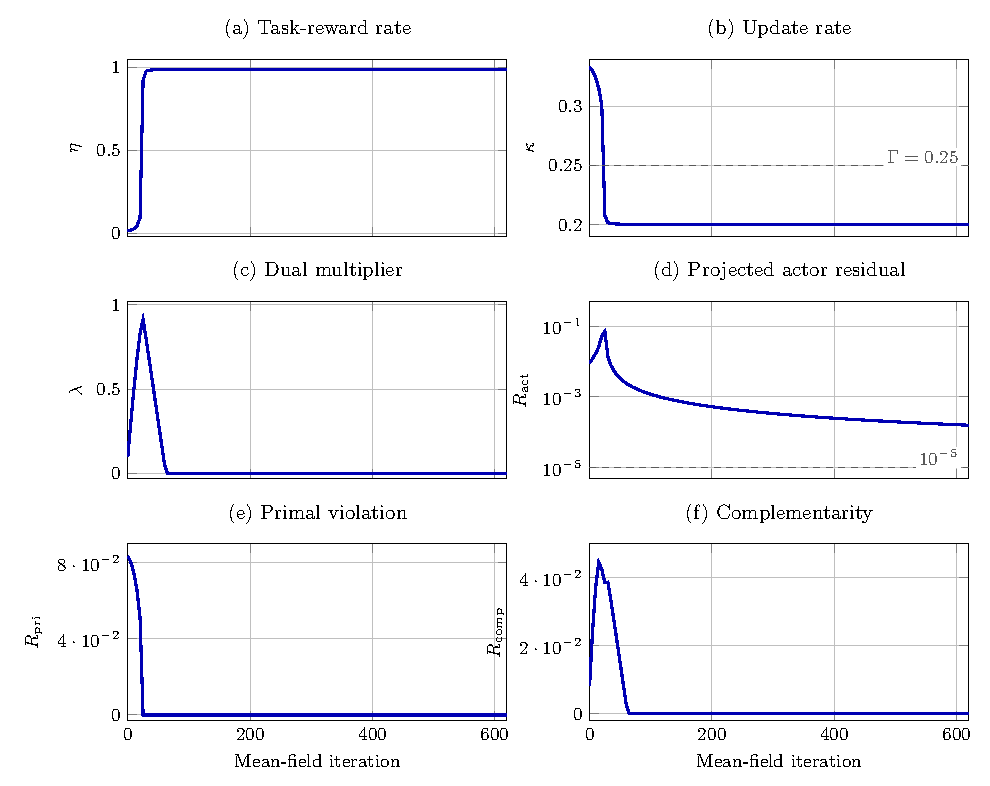
\includegraphics[width=0.92\textwidth]{figures/lactose_meanfield_trace.pdf}
\caption{Exact-model lactose mean-field diagnostic at $\Gamma_{\rm lac}^{\rm conv}=0.25$. The six panels show task-reward rate, update rate, multiplier, projected actor residual, primal violation, and complementarity for the same saved stochastic actors. The actor residual uses a logarithmic axis and remains above the dashed $10^{-5}$ diagnostic threshold at iteration 620. Feasibility and zero complementarity do not establish stationarity. Displayed data are every fifth iterate of the complete constant-gain trace. This calculation is separate from the first-arrival study and has no sampling-error band.}
\label{comp:fig:lactose_convergence}
\end{figure}

Table~\ref{comp:tab:heterogeneous_dwell_bootstrap} reports percentile intervals from 20,000 whole-training-seed resamples of the ten saved stochastic endpoints. The stored SeedSequence key is $(20260917,12,50,3,0,300,0,0,3)$, with PCG64 and linear quantile interpolation. Each bootstrap draw uses the same seed indices across metrics, greedy extractions and contrasts, with exact references fixed. All means and differences are formed from unrounded values; standard deviations use divisor nine. The intervals describe training-outcome variation, not rollout noise, model uncertainty or convergence error. The greedy means differ from the stochastic means by less than $4\times10^{-9}$ in occupancy and update rate, but their policy identities and evaluations remain separate. Table~\ref{comp:tab:heterogeneous_dwell_policy_counts} counts greedy actions across seeds, not state visits or randomized-action probabilities. Its statewise modes need not form a policy attaining the aggregate mean.

\begin{table}[htbp]
\caption{Uncertainty across ten exactly evaluated stochastic PD-SMAC endpoints. The unrestricted references are objective-matched. Gaps are learned values minus the named reference.}
\label{comp:tab:heterogeneous_dwell_bootstrap}
\centering
\begingroup
\small
\setlength{\tabcolsep}{3pt}
\renewcommand{\arraystretch}{1.15}
\begin{tabular*}{\linewidth}{@{\extracolsep{\fill}}>{\raggedright\arraybackslash}p{0.46\linewidth}ccc@{}}
\toprule
Quantity & Mean & \shortstack{Sample\\standard deviation} & \shortstack{Bootstrap 95\%\\confidence interval} \\
\midrule
Target occupancy & $0.961092$ & $0.010276$ & $[0.954643,0.966940]$ \\
Task-reward rate & $0.960050$ & $0.010708$ & $[0.953298,0.966103]$ \\
Update rate & $0.247135$ & $0.025124$ & $[0.231304,0.262089]$ \\
Stationary mean hold & $4.087924$ & $0.454218$ & $[3.815796,4.376608]$ \\
Update-rate residual & $-0.052865$ & $0.025124$ & $[-0.068696,-0.037911]$ \\
Occupancy minus best feasible fixed-$\tau$ reference & $0.034810$ & $0.010276$ & $[0.028362,0.040658]$ \\
Occupancy minus deterministic reference & $-0.007386$ & $0.010276$ & $[-0.013835,-0.001538]$ \\
Occupancy minus unrestricted occupancy LP & $-0.011570$ & $0.010276$ & $[-0.018019,-0.005722]$ \\
Reward minus unrestricted penalized LP & $-0.011877$ & $0.010708$ & $[-0.018629,-0.005824]$ \\
\bottomrule
\end{tabular*}
\endgroup
\end{table}

\begin{table}[htbp]
\caption{Statewise action counts across the ten final greedy PD-SMAC policies in the heterogeneous-dwell diagnostic. The state labels are $S$ for the safe target state, $B$ for the boundary target state, $O$ for the off-target state, and $L$ for the latent off-target state.}
\label{comp:tab:heterogeneous_dwell_policy_counts}
\centering
\small
\resizebox{\textwidth}{!}{%
\begin{tabular}{llccc}
\toprule
State & Modal learned macro-action & Modal count & Long holds $\tau\ge4$ & Short holds $\tau\le2$ \\
\midrule
$S$ safe target & $(u,\tau)=(0,4)$ & $7/10$ & $10/10$ & $0/10$ \\
$B$ boundary target & $(u,\tau)=(1,1)$ & $9/10$ & $1/10$ & $9/10$ \\
$O$ off target & $(u,\tau)=(1,2)$ & $8/10$ & $2/10$ & $8/10$ \\
$L$ latent off target & $(u,\tau)=(1,3)$ & $5/10$ & $0/10$ & $5/10$ \\
\bottomrule
\end{tabular}}
\end{table}

\paragraph{Continuing and sensitivity evidence.}
Tables~\ref{comp:tab:continuing_endpoints}--\ref{comp:tab:saved_policy_diagnostics} retain primary and secondary modes separately. For the continuing cohort, 20,000 whole-seed percentile resamples with linear quantiles give the final stochastic reward interval
\[
 [0.555321400394,0.562250742410].
\] These descriptive intervals are not simultaneous coverage claims or tests of asymptotic convergence. The 28-node contrast resamples the four within-path differences; reused fixed references do not acquire trained-seed deviations.

\begin{table}[htbp]
\caption{Continuing four-state endpoints after $10^6$ complete decisions per seed. Rates and deviations are computed from ten stationary saved-policy evaluations. Values are mean $\pm$ sample standard deviation. The stochastic row is primary. The greedy maps have no inherited actor or multiplier certificate; only the stochastic policies carry the diagnostics below.}
\label{comp:tab:continuing_endpoints}
\centering\begingroup\small
\setlength{\tabcolsep}{3pt}
\begin{tabular*}{\linewidth}{@{\extracolsep{\fill}}lcccc@{}}
\toprule
Policy & Target occupancy & Task reward & Update rate & Feasible seeds \\
\midrule
Stochastic & $0.568701\pm0.005811$ & $0.558343\pm0.005969$ & $0.327455\pm0.001490$ & 0/10 \\
Greedy & $0.929183\pm0.007752$ & $0.926353\pm0.008241$ & $0.215062\pm0.018074$ & 10/10 \\
\bottomrule
\end{tabular*}
\par\smallskip
\begin{tabular*}{\linewidth}{@{\extracolsep{\fill}}lccc@{}}
\toprule
Stochastic diagnostic & Mean & Minimum & Maximum \\
\midrule
$\lambda$ & $0.299313$ & $0.196823$ & $0.379040$ \\
$R_{\rm act}$ & $0.091731$ & $0.088950$ & $0.097163$ \\
$R_{\rm adv}$ & $2.073806$ & $2.042679$ & $2.129584$ \\
$R_{\rm pri}$ & $0.027455$ & $0.024146$ & $0.029215$ \\
$R_{\rm comp}$ & $0.008273$ & $0.004752$ & $0.011006$ \\
\bottomrule
\end{tabular*}
\endgroup
\end{table}

\begin{table}[htbp]
\caption{Paired training-budget 28-node control. Each learned entry is a mean $\pm$ sample standard deviation across four paths, with 120 paired evaluation rollouts per path. Primary comparisons use greedy policies. The lower block gives within-path occupancy changes from episode 240 to 1200 and unadjusted 95\% percentile intervals from 20,000 whole-path resamples. Secondary stochastic modes are not substituted for primary rows.}
\label{comp:tab:training_budget_sensitivity}
\centering\begingroup\footnotesize
\setlength{\tabcolsep}{2pt}
\renewcommand{\arraystretch}{1.13}
\begin{tabular*}{\linewidth}{@{\extracolsep{\fill}}lcccc@{}}
\toprule
Policy & \shortstack{Occupancy\\240 episodes} & \shortstack{Occupancy\\1200 episodes} & \shortstack{Task reward\\1200 episodes} & \shortstack{Update rate\\1200 episodes} \\
\midrule
DDQN+PER, greedy & $0.379911\pm0.176681$ & $0.616443\pm0.040297$ & $0.593546\pm0.032093$ & $1.000000\pm0.000000$ \\[2pt]
TT-AC, greedy & $0.083333\pm0.028260$ & $0.518824\pm0.276882$ & $0.481833\pm0.252607$ & $1.000000\pm0.000000$ \\[2pt]
TT-AC, stochastic & $0.416518\pm0.108934$ & $0.552827\pm0.200598$ & $0.513568\pm0.177669$ & $1.000000\pm0.000000$ \\[2pt]
PD-SMAC, greedy & $0.662574\pm0.019172$ & $0.662054\pm0.018657$ & $0.632594\pm0.019108$ & $0.234747\pm0.014019$ \\[2pt]
PD-SMAC, stochastic & $0.590476\pm0.041945$ & $0.653720\pm0.023528$ & $0.619381\pm0.024434$ & $0.263690\pm0.009919$ \\[2pt]
\bottomrule
\end{tabular*}
\par\smallskip
\begin{tabular*}{\linewidth}{@{\extracolsep{\fill}}lcc@{}}
\toprule
Policy & Mean paired occupancy change & 95\% percentile interval \\
\midrule
DDQN+PER, greedy & $0.236533$ & $[0.098958,0.374107]$ \\
TT-AC, greedy & $0.435491$ & $[0.145387,0.589583]$ \\
TT-AC, stochastic & $0.136310$ & $[-0.061458,0.332292]$ \\
PD-SMAC, greedy & $-0.000521$ & $[-0.001562,0.000000]$ \\
PD-SMAC, stochastic & $0.063244$ & $[0.045833,0.083333]$ \\
\bottomrule
\end{tabular*}
\par\smallskip\raggedright The fixed $u=1$, nominal-hold-5 reference has occupancy $0.662574$ with population standard deviation $0.180545$ across 480 rollouts, rate $6/28$, and realized mean hold $28/6$. It has no training-seed uncertainty and is not resimulated for this control.
\endgroup
\end{table}

\begin{table}[htbp]
\caption{Same-policy diagnostics of the ten reset/annealed stochastic endpoints. Every row uses its owned multiplier, stored temperature and penalized task reward. All are feasible and have $R_{\rm act}<10^{-5}$; seeds 1, 4 and 5 fail the $10^{-6}$ complementarity threshold. These are exact-model numerical evaluations, not additional training replications.}
\label{comp:tab:saved_policy_diagnostics}
\centering\begingroup\small
\begin{tabular*}{\linewidth}{@{\extracolsep{\fill}}ccccc@{}}
\toprule
Seed & $\lambda$ & $R_{\rm act}$ & $R_{\rm adv}$ & $R_{\rm comp}$ \\
\midrule
0 & $0.000000$ & $6.80763\times10^{-14}$ & $0.150846$ & $0.000000$ \\
1 & $0.004985$ & $1.12353\times10^{-10}$ & $0.036313$ & $0.000181$ \\
2 & $0.000000$ & $1.54692\times10^{-9}$ & $0.088664$ & $0.000000$ \\
3 & $0.000000$ & $4.85496\times10^{-11}$ & $0.038792$ & $0.000000$ \\
4 & $0.029908$ & $9.41271\times10^{-12}$ & $0.042898$ & $0.002521$ \\
5 & $0.034893$ & $4.09071\times10^{-11}$ & $0.022245$ & $0.001245$ \\
6 & $0.000000$ & $2.36095\times10^{-13}$ & $0.040188$ & $0.000000$ \\
7 & $0.000000$ & $1.10674\times10^{-7}$ & $0.148674$ & $0.000000$ \\
8 & $0.000000$ & $2.76062\times10^{-13}$ & $0.040188$ & $0.000000$ \\
9 & $0.000000$ & $4.27450\times10^{-11}$ & $0.040188$ & $0.000000$ \\
\bottomrule
\end{tabular*}
\endgroup
\end{table}


\renewcommand{\arraystretch}{1.05}

\section*{C4. Computational material, access, and reproduction scope}
\label{comp:sec:access}
The computational records distinguish saved-result aggregation, evaluation of saved policies, new training, saved-certificate verification, and fresh constrained optimization. A successful saved-certificate check does not establish that a new optimization was performed. Checkpoints of one training stream are not independent training seeds; validation replays and failed or interrupted runs are not additional replications.

The four-state and lactose models are specified algorithmically and require no external biological input file. The biological implementations require exact, authorized local inputs. File fingerprints establish identity, not ownership, permission, or a complete derivation. The 70-node discrepancy described in Section~C2.5 remains unresolved. Expression data, fitted model banks, and state-bearing biological trajectories are not authorized for public redistribution merely by preparation of this guide. Project-code licensing and permissions for derived outputs remain separate decisions.

Continuation eligibility requires the complete recorded numerical-environment match, not processor agreement alone. The existing authorization guard must remain effective. Installed-environment successes are distinct from a genuinely isolated installation; the recorded isolated attempt failed at package-index access and did not establish a clean numerical installation. This guide makes no new training, continuation, installation, or optimization claim.

The main paper and this guide identify the scientific case, estimand, cohort, uncertainty unit, and limitations of each reported comparison. The numerical implementation retains the corresponding configurations and execution records. Access terms and citation metadata accompany the software distribution. Computational agreement does not grant input or output redistribution rights.


\section*{C5. Extended numerical comparisons}
\label{comp:sec:extended_comparisons}
This section supplies the detailed reference interpretation and additional 28-node comparisons underlying the main paper. It retains the distinctions between stationary evaluations, paired finite-horizon trajectories and stochastic/greedy policy modes.

\subsection*{C5.1 Four-state references and exact policy differences}
The stochastic and greedy rows remain distinct despite coincident three-decimal entries. Their absolute mean differences are approximately $1.12\times10^{-9}$ for occupancy, $1.19\times10^{-9}$ for reward, $3.92\times10^{-9}$ for update rate and $8.97\times10^{-8}$ for mean hold. Section~C2.3 also reports their separate deviation differences. Duration 3 has slightly higher occupancy but lower penalized reward than duration 4; its rate $1/3>0.30$ makes it infeasible. Thus duration 4 remains the best feasible fixed-duration reference for this comparison.

The best feasible deterministic occupancy is $0.968478$. The two relevant maps tie exactly in occupancy and reward; the generic tolerance-aware tie rule selects the lower-rate member in main Table~\ref*{tab:heterogeneous_dwell_main}, with rate $0.276403$ and mean hold $3.617902$. They differ only at $L$, where holds 1 and 2 under input 1 give the same physical-input sequence for the additional step. Indeed, $P_1(L,S)=0$, and every possible intermediate state still selects input 1. The longer hold skips one redundant decision.

The unrestricted occupancy optimum is $0.972661989$, whereas the optimal penalized reward is $0.971927386$. Both LPs recover a policy that randomizes at $S$ between $(0,3)$ and $(0,4)$ with probabilities $0.522865$ and $0.477135$, respectively, and uses $(1,1)$ at $B$ and $(1,2)$ at $O,L$. This conditional randomization at decision epochs uses the full update budget and adjusts safe-state residence between two integer holds. It is not interpolation between plotted deterministic policy rates. The recovered zero action probabilities also distinguish this reference from a finite-logit full-support actor.

\subsection*{C5.2 28-node endpoints, checkpoints and budget sweep}
We evaluate the saved greedy policies every 40 episodes using 120 rollouts per seed. Common reset and plant-randomness tapes pair the methods and budgets, independently of training. The episode-240 evaluations supply both main Table~\ref*{tab:melanoma28_main} and the terminal points of Fig.~\ref{comp:fig:melanoma28_curves}, without a separate holdout or endpoint selection. Stochastic actors are evaluated separately. 

\begin{figure}[htbp]
\centering
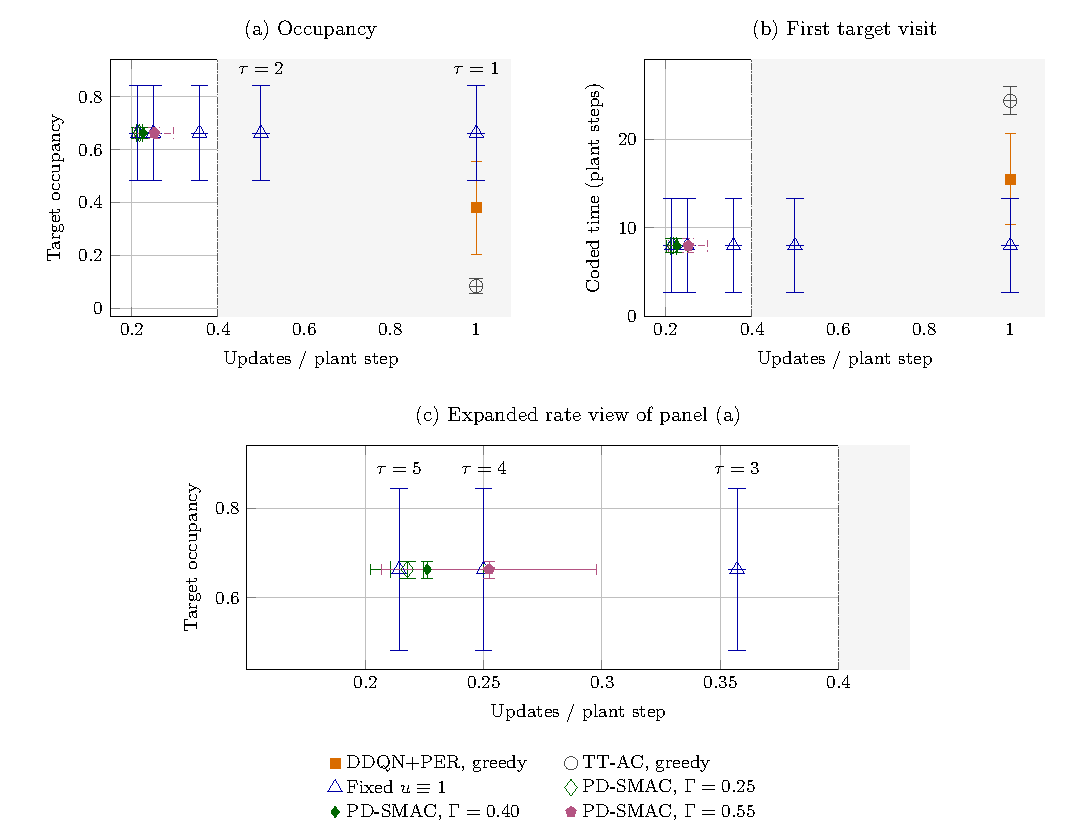
\includegraphics[width=0.96\textwidth]{figures/Figure_2_melanoma28_tradeoff.pdf}
\caption{28-node XOR-pirin endpoint comparisons. Learned bars are sample standard deviations across four training-seed means; fixed-hold bars are population standard deviations across 480 rollouts. Triangles mark $u\equiv1$ holds $1,\ldots,5$ and distinct diamond/pentagon markers the three greedy PD-SMAC budgets. Labels identify scheduled fixed holds. The expanded-rate panel resolves the low-rate policies without jitter. All points denote evaluated policies; no segments interpolate between discrete controllers. The line and shading refer to $\Gamma=0.40$. Coded first-target times include failure code 29. The fixed-hold family is horizontal in occupancy--rate coordinates.}
\label{comp:fig:melanoma28_tradeoff}
\end{figure}

\begin{figure}[htbp]
\centering
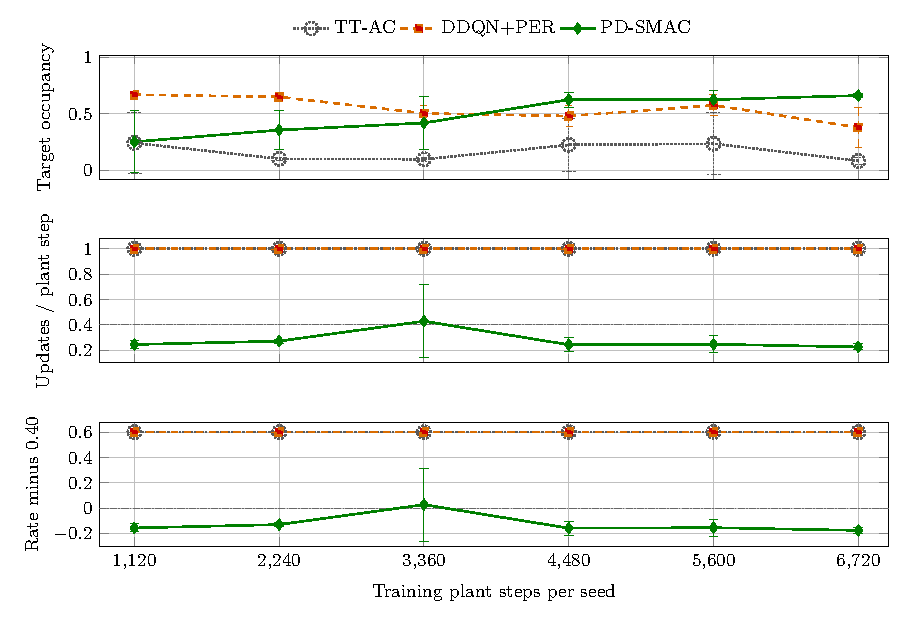
\includegraphics[width=0.96\textwidth]{figures/Figure_3_melanoma28_learning_curves.pdf}
\caption{28-node greedy checkpoint evaluations at $\Gamma=0.40$. Means and sample standard deviations use four training seeds, each with 120 evaluation rollouts. The horizontal axis counts training plant steps per seed; episode $e$ corresponds to $28e$ steps. The terminal evaluation records are exactly those in main Table~\ref*{tab:melanoma28_main}. DDQN+PER and TT-AC coincide at update rate one and residual $+0.60$; their distinct markers share those coordinates. Lines connect successive checkpoints, not asymptotic convergence certificates.}
\label{comp:fig:melanoma28_curves}
\end{figure}

\begin{table}[htbp]
\caption{28-node PD-SMAC budget sweep for saved greedy policies. Entries are means $\pm$ sample standard deviations across four training seeds. The common target occupancy is $0.663\pm0.019$ across the same four seedwise evaluation means. All three budgets have the same observed target trajectories, but their inputs, rewards and schedules need not coincide. The last column counts seedwise empirical feasibility, not stochastic-actor feasibility.}
\label{comp:tab:melanoma28_budget_sweep}
\centering
\begingroup
\fontsize{8}{10}\selectfont
\setlength{\tabcolsep}{2pt}
\renewcommand{\arraystretch}{1.14}
\begin{tabular*}{\linewidth}{@{\extracolsep{\fill}}cccccc@{}}
\toprule
$\Gamma$ & \shortstack{Task\\reward} & \shortstack{Update\\rate} & \shortstack{Realized\\hold} & \shortstack{Rate\\residual} & \shortstack{Feasible\\seeds} \\
\midrule
$0.25$ & \shortstack{$0.607$\\$\pm0.025$} & \shortstack{$0.218$\\$\pm0.007$} & \shortstack{$4.595$\\$\pm0.143$} & \shortstack{$-0.032$\\$\pm0.007$} & 4/4 \\[2pt]
$0.40$ & \shortstack{$0.610$\\$\pm0.018$} & \shortstack{$0.226$\\$\pm0.024$} & \shortstack{$4.455$\\$\pm0.424$} & \shortstack{$-0.174$\\$\pm0.024$} & 4/4 \\[2pt]
$0.55$ & \shortstack{$0.610$\\$\pm0.023$} & \shortstack{$0.252$\\$\pm0.046$} & \shortstack{$4.052$\\$\pm0.658$} & \shortstack{$-0.298$\\$\pm0.046$} & 4/4 \\[2pt]
\bottomrule
\end{tabular*}
\endgroup
\end{table}

The constant-input identity gives the same regulation statistics at all five fixed holds, with update rates $1$, $1/2$, $10/28$, $7/28$ and $6/28$. Holds $3,4,5$ satisfy $\Gamma=0.40$. main Table~\ref*{tab:melanoma28_main} reports their common regulation statistics once, using the longest hold for its accounting columns; Fig.~\ref{comp:fig:melanoma28_tradeoff} retains every duration-specific rate.

At 3360 training plant steps (episode 120), the greedy PD-SMAC mean update rate is $0.429\pm0.287$, above $0.40$. The feasible terminal values do not imply budget satisfaction at every checkpoint.

\begingroup\clubpenalty=10000

All twelve greedy endpoints satisfy their empirical budgets. However, stochastic seed 2 at $\Gamma=0.25$ has rate $0.254167$, above budget despite the four-seed mean $0.245238$. Feasibility therefore remains policy-specific; the extracted greedy policy does not certify the stochastic actor owning the multiplier. Main Section~6.4 distinguishes these finite-reset feature experiments from the stationary theory.


\endgroup

\subsection*{C5.3 Persistent-input duration accounting}
The paired terminal 70-node evaluations apply the same constant input under every fixed duration. Table~\ref{comp:tab:persistent_duration_accounting} reports the complete update accounting used with the endpoint results in main Table~\ref*{tab:bittner70_main}. A nominal hold of six is executed as $6,6,6,2$, producing four updates and a realized mean hold of five. Figure~\ref{comp:fig:melanoma70_tradeoff} presents the saved endpoint coordinates at full and expanded rate scales; no fitted or interpolated policy is added.

\begin{table}[tbp]
\caption{70-node fixed-input duration accounting at horizon $H=20$ and update budget $0.40$. Every row uses the same constant input and paired plant trajectories. Scheduled and realized holding times differ when the last interval is truncated.}
\label{comp:tab:persistent_duration_accounting}
\centering
\begingroup\small
\begin{tabular*}{\linewidth}{@{\extracolsep{\fill}}cccccc@{}}
\toprule
Scheduled $\tau$ & Updates $K_H$ & Realized hold & Update rate & Rate residual & Within budget \\
\midrule
$1$ & $20$ & $1.000$ & $1.000$ & $+0.600$ & No \\
$2$ & $10$ & $2.000$ & $0.500$ & $+0.100$ & No \\
$4$ & $5$ & $4.000$ & $0.250$ & $-0.150$ & Yes \\
$6$ & $4$ & $5.000$ & $0.200$ & $-0.200$ & Yes \\
\bottomrule
\end{tabular*}
\endgroup
\end{table}

\begin{figure}[tbp]
\centering
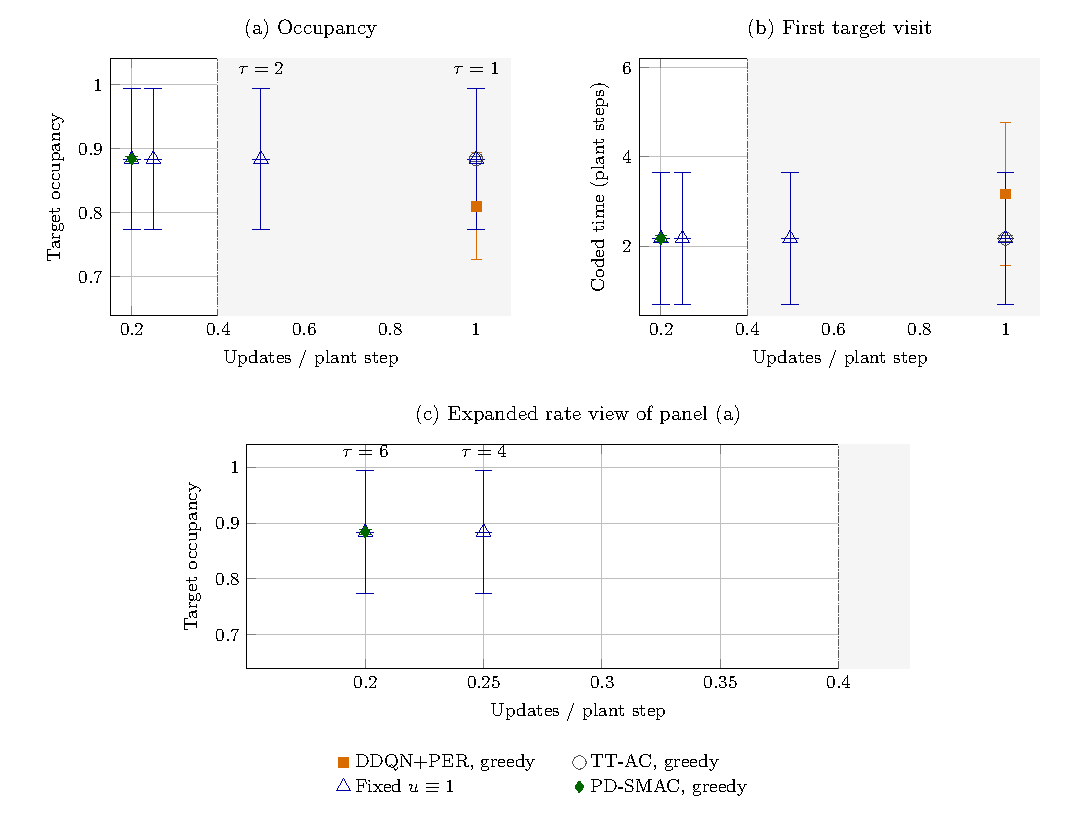
\includegraphics[width=0.96\textwidth]{figures/melanoma70_endpoints.pdf}
\caption{70-node force-pirin comparison from the final saved policies. Learned bars are sample standard deviations across five training-seed means; periodic bars are population standard deviations across 1500 rollouts. Open triangles identify nominal holds $1,2,4,6$ under $u\equiv1$, at rates $1,0.5,0.25,0.2$. TT-AC and PD-SMAC coincide with the nominal-1 and nominal-6 reference means, respectively. The vertical line and shading identify $\Gamma=0.40$ and larger rates. Points are not joined into unattested interpolated policies. Panel (b) uses failure-coded first-target time. Panel (c) expands the rate axis of panel (a), with identical coordinates and error bars.}
\label{comp:fig:melanoma70_tradeoff}
\end{figure}

\end{document}
